\chapter{Physical Properties of CO emitters}

\section{Previous Work}

There have been two main types of surveys for searching for CO emitters in the universe, targeted and blind surveys. In targeted surveys, targets are chosen based on some type of preselection, such as star formation rate, mass, or some other parameter \cite{walter2016alma, decarli2019alma}, and are looked at specifically to see what CO emissions can be found in that galaxy or galaxies. While these surveys have given useful information on the role gas plays in these galaxies, the preselection process means that there could be a bias in our knowledge of CO. For example, these surveys could miss out on dark, gas-rich galaxies that are hard to detect, giving us an incomplete picture of the variety of galaxies with gas and CO emission in the universe. 

Blind surveys are the opposite of targeted surveys. Instead of choosing the targets and looking at them specifically, blind surveys choose an area of the sky and search for any CO emissions within that cosmic volume, allowing for any emissions above the sensitivity limit of the survey to be found. This allows for a sort of census of all the gas within a cosmic volume \cite{decarli2019alma}. 

Previous blind surveys include the COLDz survey in the GOODS-North region, the PdBI survey, as well as the first two surveys in the ASPECS program, ASPECS Pilot and ASPECS Large Program. 

The PdBI survey was a molecular line survey in the Hubble Deep Field North (HDF-N) in 3mm using the IRAM Plateau de Bure Interferometer (PdBI) \cite{decarli2014molecular}. This survey was designed to cover all CO transitions detectable above z $>$ 2, and well as covering the redshift ranges of z $<$ 0.45, and 1 $<$ z $<$ 1.9. The survey identified 17 line candidates, with most of the candidates falling in intermediate redshifts (z $<$ 3), and with 7 of the line candidates matching to galaxies in their catalog \cite{decarli2014molecular}. 

COLDz, or the CO Luminosity Density at High-z (COLDz) targeted CO(1-0) emissions from galaxies at redshifts between 1.95-2.85 and CO(2-1) emission between z = 4.91 - 6.70 using the Very Large Array (VLA)\cite{pavesi2018co}. This survey covers a wide area of around 51 arcminute$^2$, as well as a roughly 9 arcminute$^2$ area much more deeply. This survey blindly selected starburst and massive main sequence galaxies in the GOODS-North and COSMOS fields. COLDz found seven secure CO line detections, and 57 above their S/N threshold, including many that did not have optical or near infrared counterparts, suggesting that those candidates could potentially be from a population of gas-rich, but optically dark galaxies \cite{pavesi2018co}.

% Add exactly how deeply it looked
The ASPECS Pilot and Large Programs both looked at regions in the Hubble Ultra Deep Field. The Pilot program looked incredibly deeply in the 1.2mm and 3mm bands at a small, one arcsecond region of the Hubble eXtremely Deep Field (XDF). The spectral coverage of the Pilot meant that it could detect CO transitions almost continuously from z = 0 to z = 8, as well as CII emissions from z = 6 to z = 8 \cite{walter2016alma}. This allowed for the characterization of CO emitters all the way to a z = 8, as well as giving constraints on the knee of the CO luminosity function \cite{walter2016alma}. 

% Add how deeply it looked, how sensetive, in decarli paper
The Large Program looked wider, but shallower, covering a roughly five square arcminute area of the Hubble Ultra Deep Field (HUDF) surrounding the ASPECS Pilot region. It was a 150 hour molecular deep field taken at 1.2mm and 3mm \cite{decarli2019alma}. The greater volume probed by the Large Program allowed for constraining the density of gas in the universe, as well as better constraints on the CO luminosity function. The survey blindly revealed the molecular gas content in normal, star-forming main-sequence galaxies \cite{decarli2019alma}. 

\section{The Wide ASPECS Survey}

The Wide ASPECS survey builds upon the Pilot and Large Program, going much wider, but also shallower. This means that Wide ASPECS cannot capture as dim CO emitters, but because of the much larger cosmic volume looked at, it can find rarer, but very bright CO emitters that did not happen to fall within the Large Program and Pilot survey bounds.
% Specify the six frequency settings range, and that it allows the detection of CO in the z ranges it does

The data for this survey was observed in ALMA Cycle 5 and was observed in Band 3 (3mm) for ~20 hours in 130 pointings and six frequency settings. The survey covered ~52.5 arcminutes$^2$ of the sky at 20\% sensitivity, and ~43 arcminutes$^2$ at 50\% sensitivity. This means Wide ASPECS covers roughly five times the area of the ASPECS Large Program. This raw data was processed with the CASA ALMA pipeline into six datacubes, one for each frequency setting.
% Add the senseitivity

\begin{figure}[tbp]
\centering 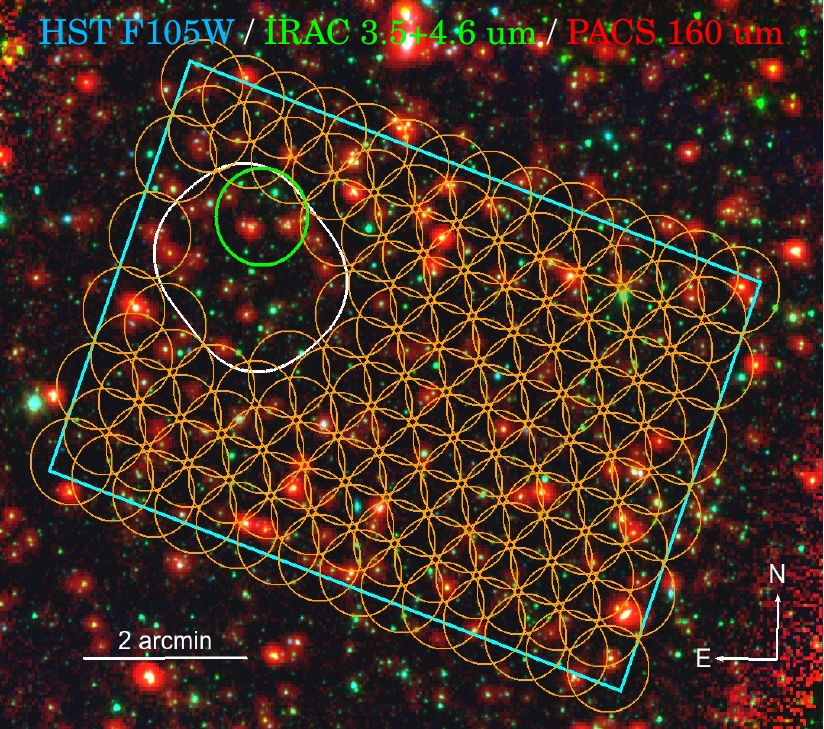
\includegraphics[width=120mm]{Wide_ASPECS_Coverage.png}
\caption{Spatial coverage of ASPECS Pilot (Green), Large Program (White), and Wide (Yellow) showing each of the individual pointings. The area covered by the Pilot is $~$1 arcmin$^2$, by the Large Program $~$5 arcmin$^2$, and by Wide ASPECS, $~$52.5 armin$^2$. The cyan box is the 50\% sensitivity extent of the survey. This region covers the area of the deepest CANDELS observations, where a wealth of ancillary data has been collected in over 30 photometric bands. Figure adapted from Decarlie et al. (in prep.)}
% Put this in the Wide ASPECS description stuff
\label{fig:ASPECS_Coverage}
\end{figure}

\begin{figure}[tbp]
\centering
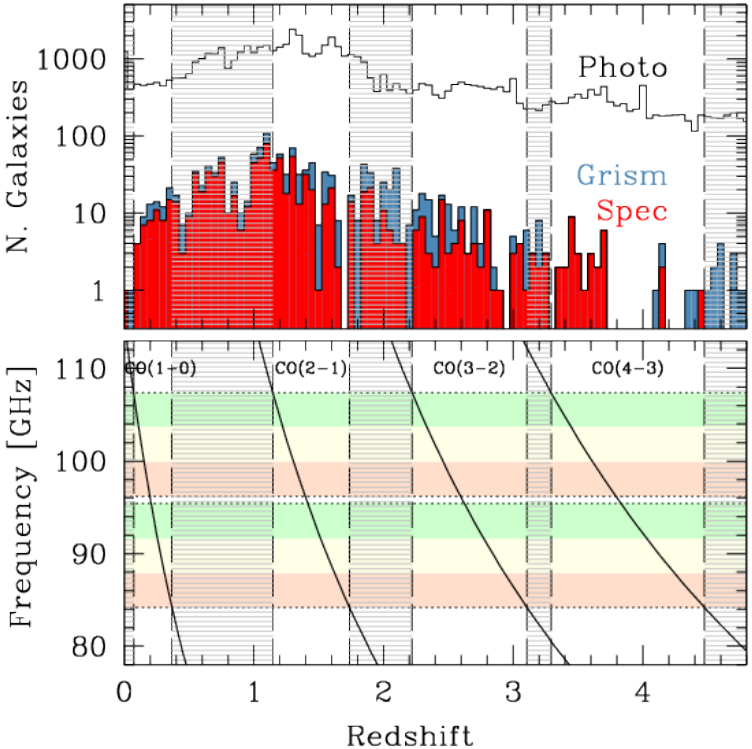
\includegraphics[width=120mm]{Wide_ASPECS_Freq.png}
\caption{Spectral and redshift coverage of Wide ASPECS in relation to the redshift distribution of galaxies within the survey field. Wide ASPECS is designed to detect CO line transitions at z$<$0.4, 1.1 $<$ z $<$ 1.8, and 2.2 $<$ z $<$ 4.4. Figure adapted from Decarlie et al. (in prep.)}
\label{fig:ASPECS_Freq}
\end{figure}

\begin{table}[]
\caption{Redshift limits and cosmic volume probed for each CO transition observable by Wide ASPECS.}
\begin{tabular}{lllll}
Transition & $z_{low}$ & $z_{high}$ & Freq. (GHz) & Volume (Mpc$^3$) \\
\hline
1-0        & 0.0030    & 0.3694     & 115.271     & 4461             \\
2-1        & 1.0059    & 1.7387     & 230.538     & 107411           \\
3-2        & 2.0088    & 3.1080     & 345.796     & 191232           \\
4-3        & 3.0115    & 3.3771     & 461.041     & 237143          
\end{tabular}
\end{table}

\subsection{Ancillary Data}\label{sec:ancillary}

In addition to each of the ALMA datacubes, there is a lot of ancillary data available as the GOODS-South region is one of the most studied regions of the sky. This data has been collected through combining multiple other catalogs, first described in \cite{walter2016alma} and expanded with new data in \cite{decarli2019alma}, comprising over 30 photometric bands for over 63000 galaxies in and around the footprint of Wide ASPECS. 26251 galaxies lie within the footprint of Wide ASPECS, of which 2283 have spectroscopic redshifts, and 23968 have photometric redshifts. 

The majority of the ancillary data comes from the Hubble Space Telescope (HST) Cosmic Assembly Near-infrared Deep Extragalactic Legacy Survey (CANDELS)\cite{grogin2011candels, Koekemoer_2011}. Most of the photometric data comes from \cite{skelton20143d}, which additionally includes ground-based optical and NIR photometry from \cite{nonino2009deep, hildebrandt2006gabods, erben2005gabods, retzlaff2010great, Hsieh_2012, 2008ApJ...682..985W, cardamone2010multiwavelength}, as well as Spitzer IRAC 3.6$\mu$m, 4.5$\mu$m, 5.8$\mu$m, and 8.0$\mu$m photometry from \cite{dickinson2003evolution, elbaz2011goods, 2013ApJ...769...80A}. There is also data from the Spitzer MIPS 24$\mu$m photometric information from \cite{Whitaker_2014}, and ALMA 1.1mm data from \cite{franco2018goods}. Additional far-infrared data from Herschel PACS at 100$\mu$m and 160$\mu$m as obtained from \cite{elbaz2011goods}. Spectroscopic redshifts came mostly from the MUSE Hubble Ultra Deep Survey \cite{bacon2017, inami2017}, while more spectroscopic information was included from \cite{le2005vimos, coe2006galaxies, skelton20143d, morris2015wfc3}. Hubble grism spectroscopy was taken from the 3D-HST survey \cite{momcheva20163d}. %All these catalogs were merged into a single catalog through matching sources within 0.5 arcseconds for the photometry, and 1.0 arcseconds for the spectroscopic data. Finally, these matches were then cross-matched with morphological parameters from \cite{van2012structural}.

%26251 in footprint of Wide ASPECS
%2283 wth Spectroscopic Z
%23968 with Photometric Z

%After > 1.99 SFR cut:

%22073
%2260
%19813

\subsection{Galaxy SED Fitting}

% Introduce the section 1.3 stuff here again

To estimate the properties of the galaxies in the catalog, the SED fitting program MAGPHYS was used \cite{da2008simple, da2015alma}. MAGPHYS computes a marginalized likelihood distribution for each of the different physical parameters of the observed galaxy through comparing the observed SED with the precomputed models. It also outputs the best-fit total SED for a given galaxy. In this report, the MAGPHYS high-z extension was used \cite{da2015alma}. % Write what makes high-z dfferent

An example output from MAGPHYS is shown in Fig. \ref{fig:MAGPHYS_Example}, showing the model, the likelihood values for various physical properties of the galaxy, and the data points used to compute the SED in red. The distribution of the stellar mass, and star formation rates of all the galaxies fitted with MAGPHYS are shown in Fig. \ref{fig:MAGPHYS_Mstar} and Fig. \ref{fig:MAGPHYS_SFR} respectively. Galaxies whose computed star formation rate was at or below a $log_{10}(SFR) = -1.99$ were removed from the rest of the analysis, as this seemed to indicate a very poor MAGPHYS fit. That left a total of around 55000 galaxies in the sample, of which 22073 were in the Wide ASPECS footprint.

\begin{figure}[tbp]
\centering 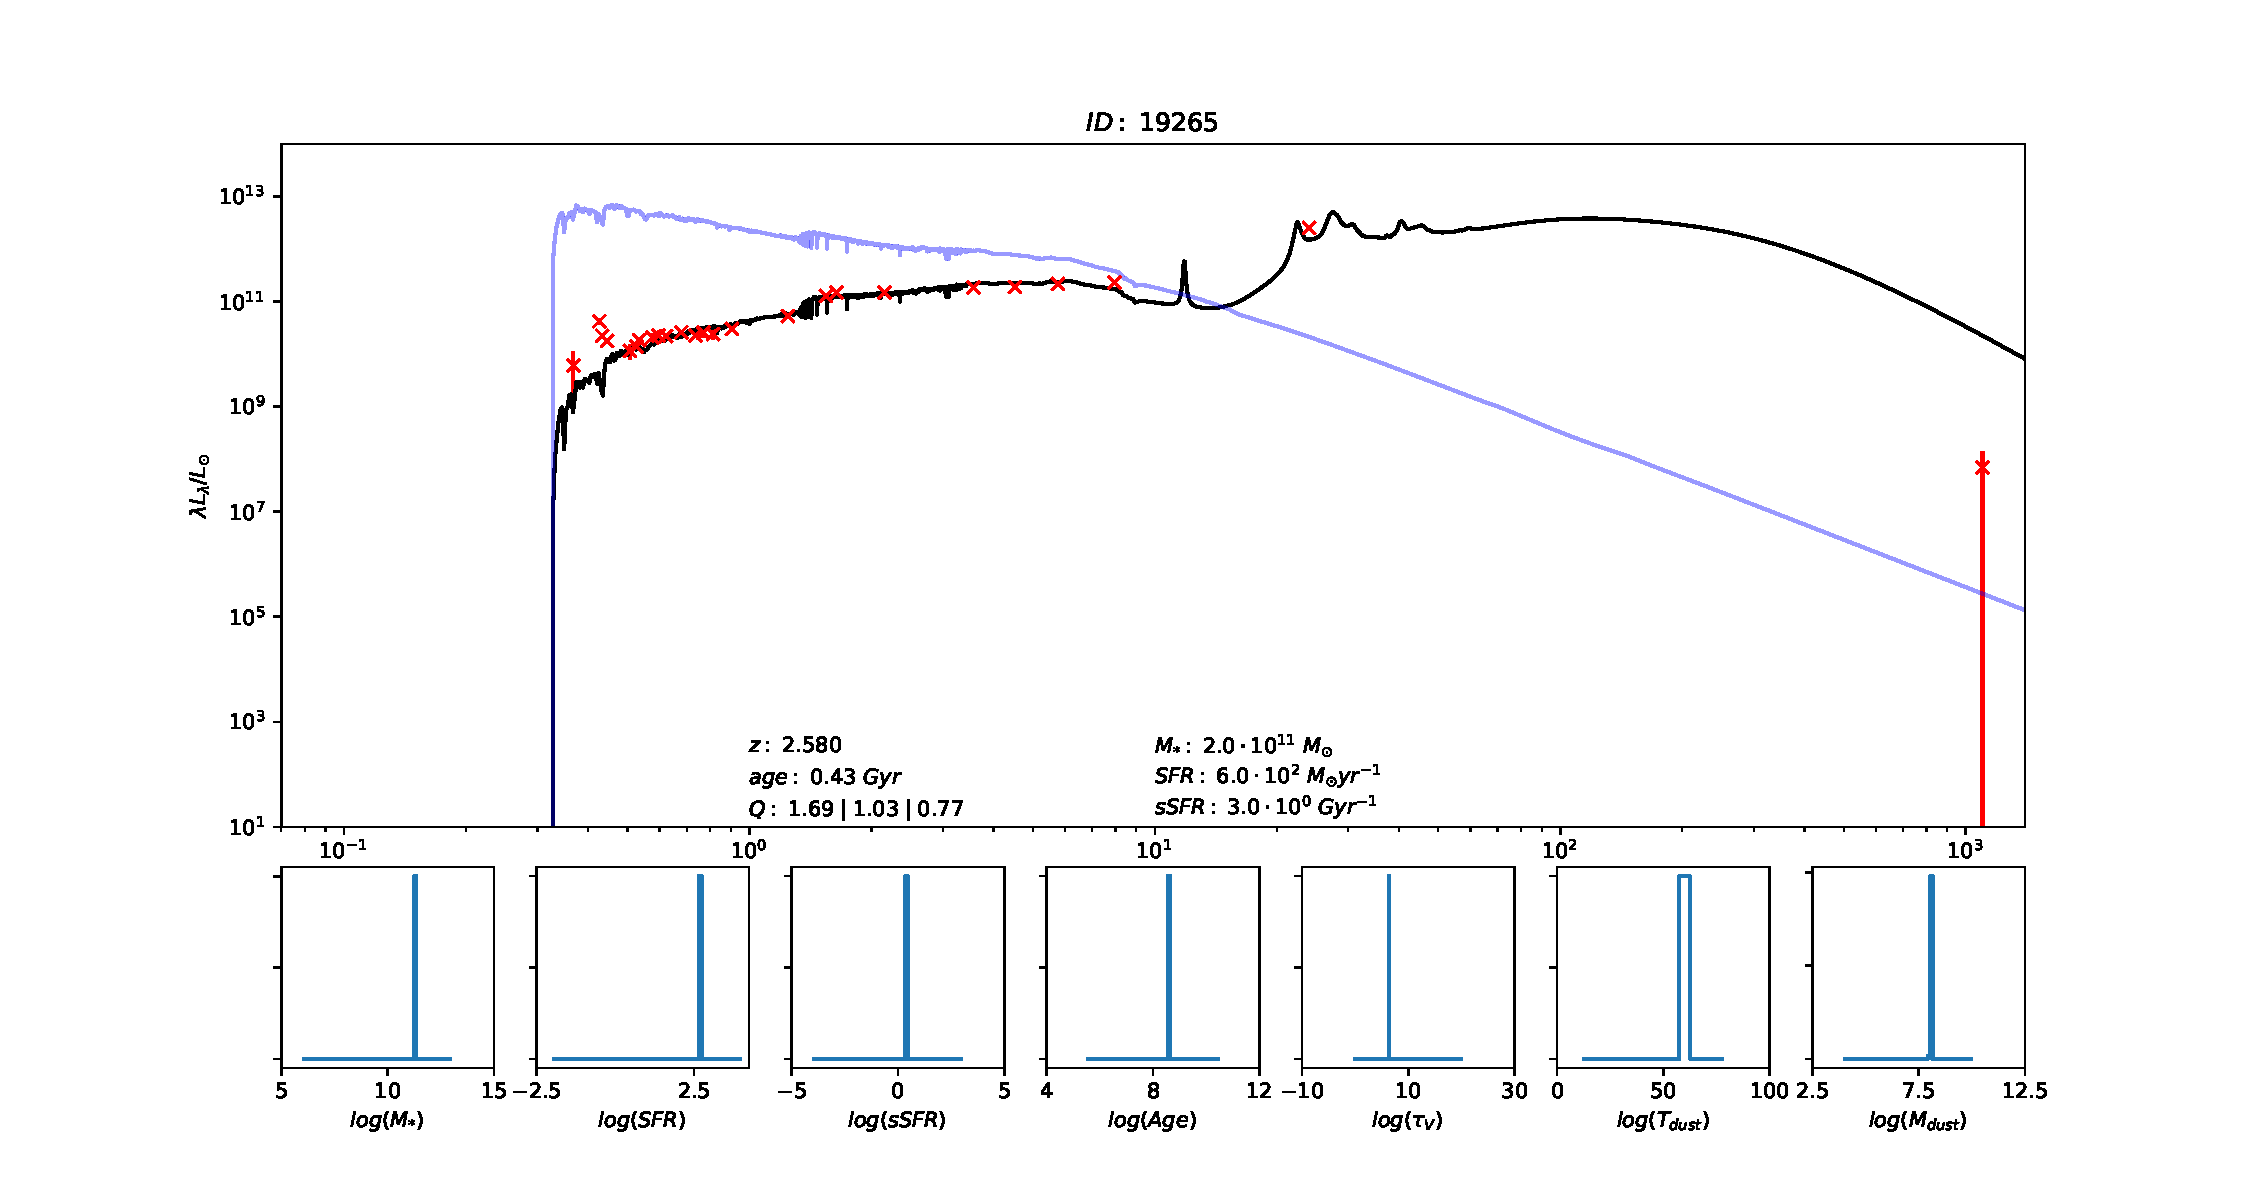
\includegraphics[width=120mm]{19265.pdf}
\caption{Example MAGPHYS output, from the most massive matched galaxy, ID.9 in Table \ref{table:Catalog}. The blue line is the spectrum of the galaxy without attenuation. The black line is the model used by MAGPHYS. The red dots are the data points. The bottom row of graphs show the probability distribution for various physical properties.}
\label{fig:MAGPHYS_Example}
\end{figure}

\begin{figure}[!tbp]
\centering 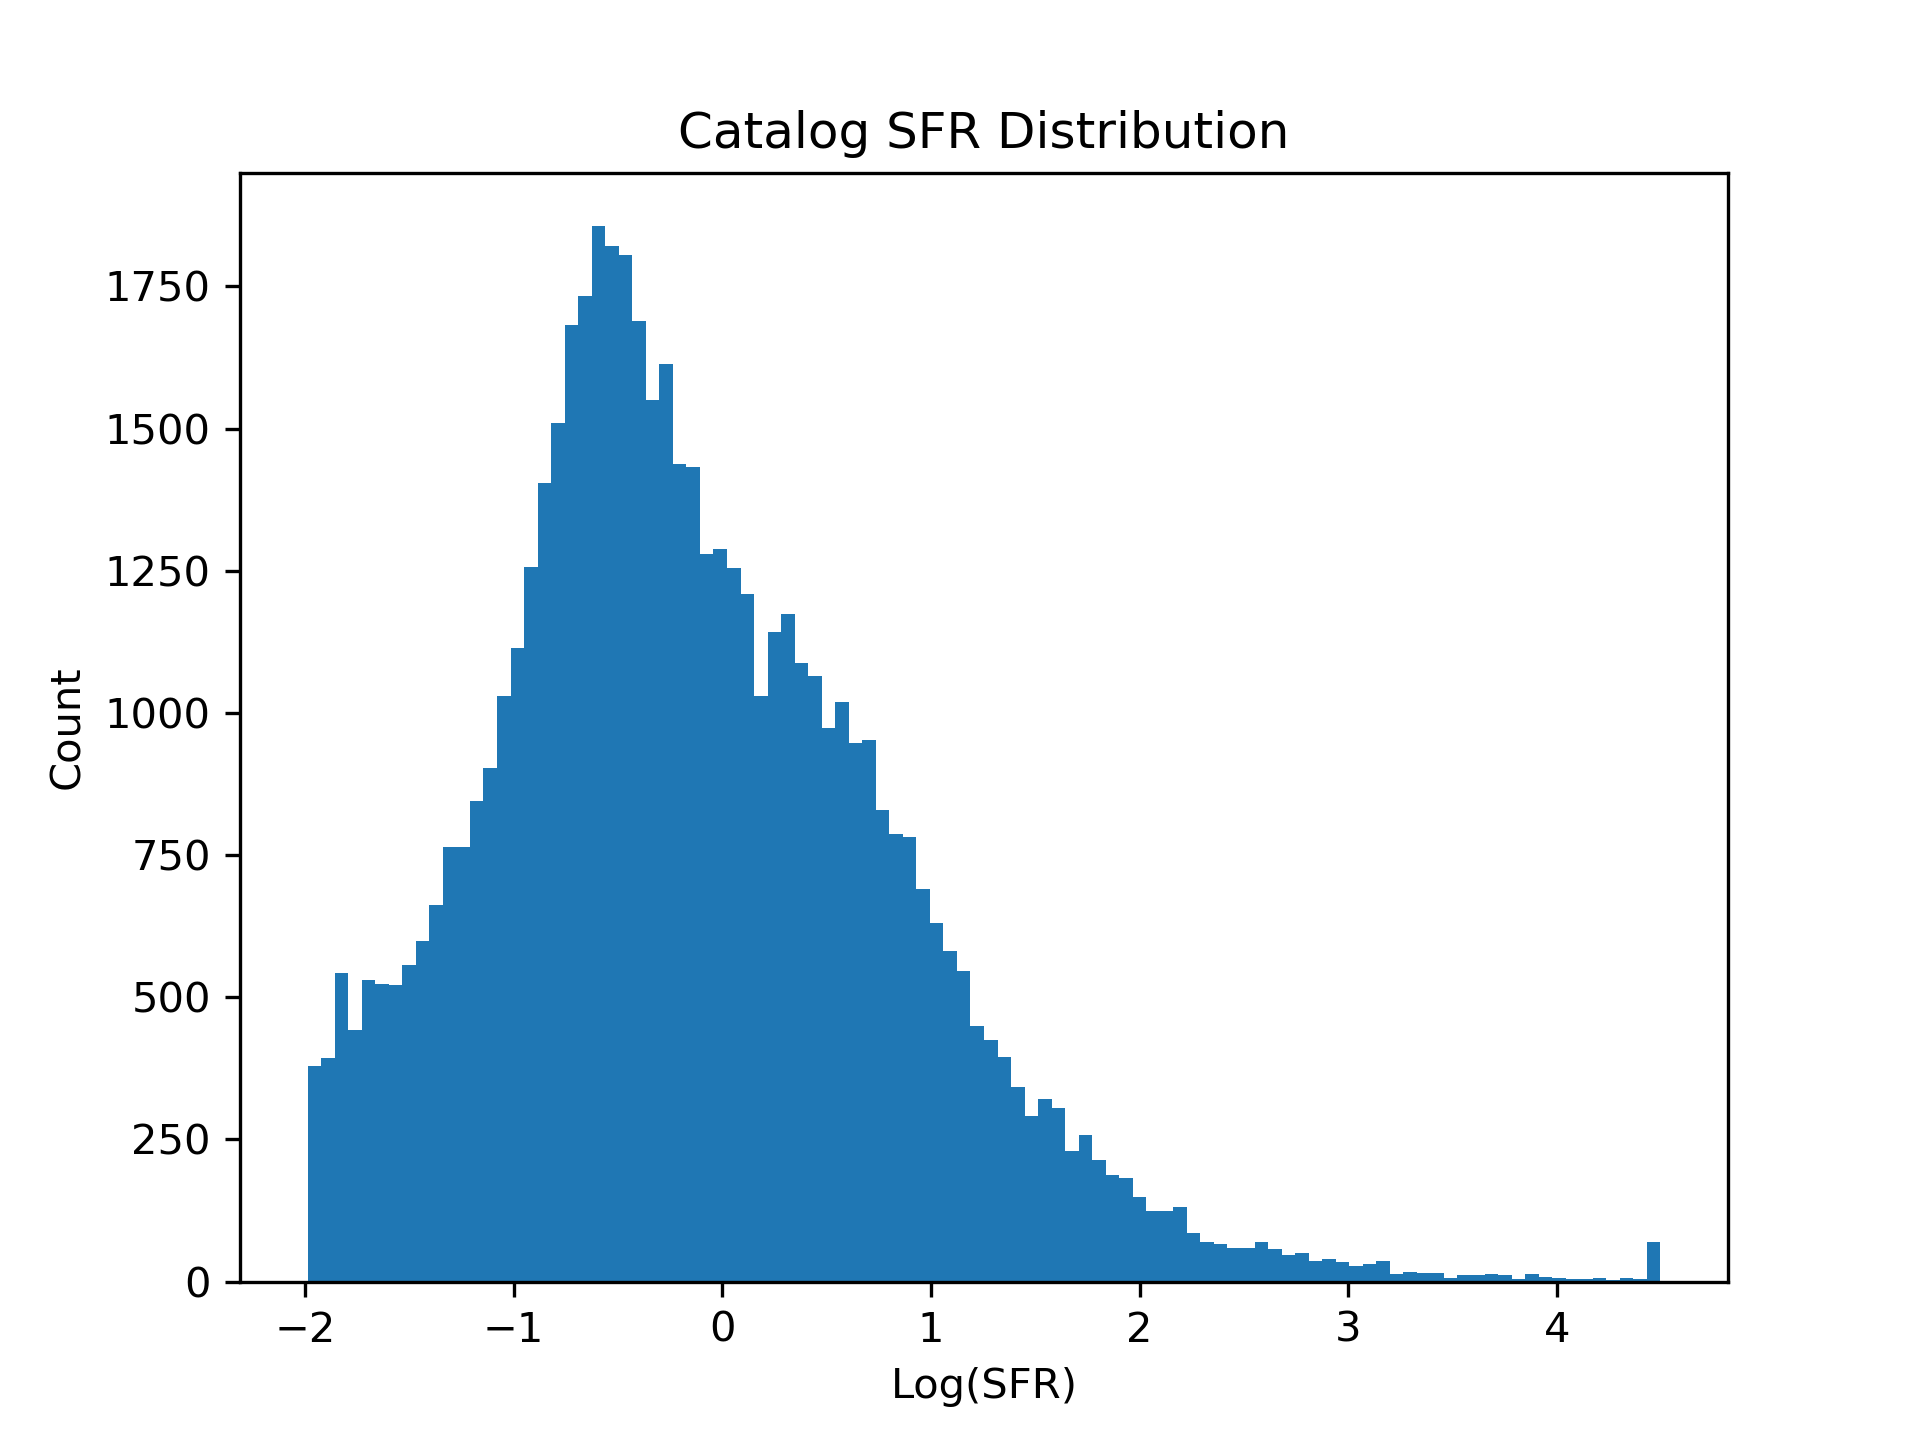
\includegraphics[width=87mm]{Survey/MAGPHYS_SFR.png}
\caption{Distribution of star formation rate for all galaxies in the catalog. The cutoff at -1.99 is from the quality cut to remove galaxies that had very poor MAGPHYS fits.}
\label{fig:MAGPHYS_SFR}
\end{figure}

\begin{figure}[!tbp]
\centering 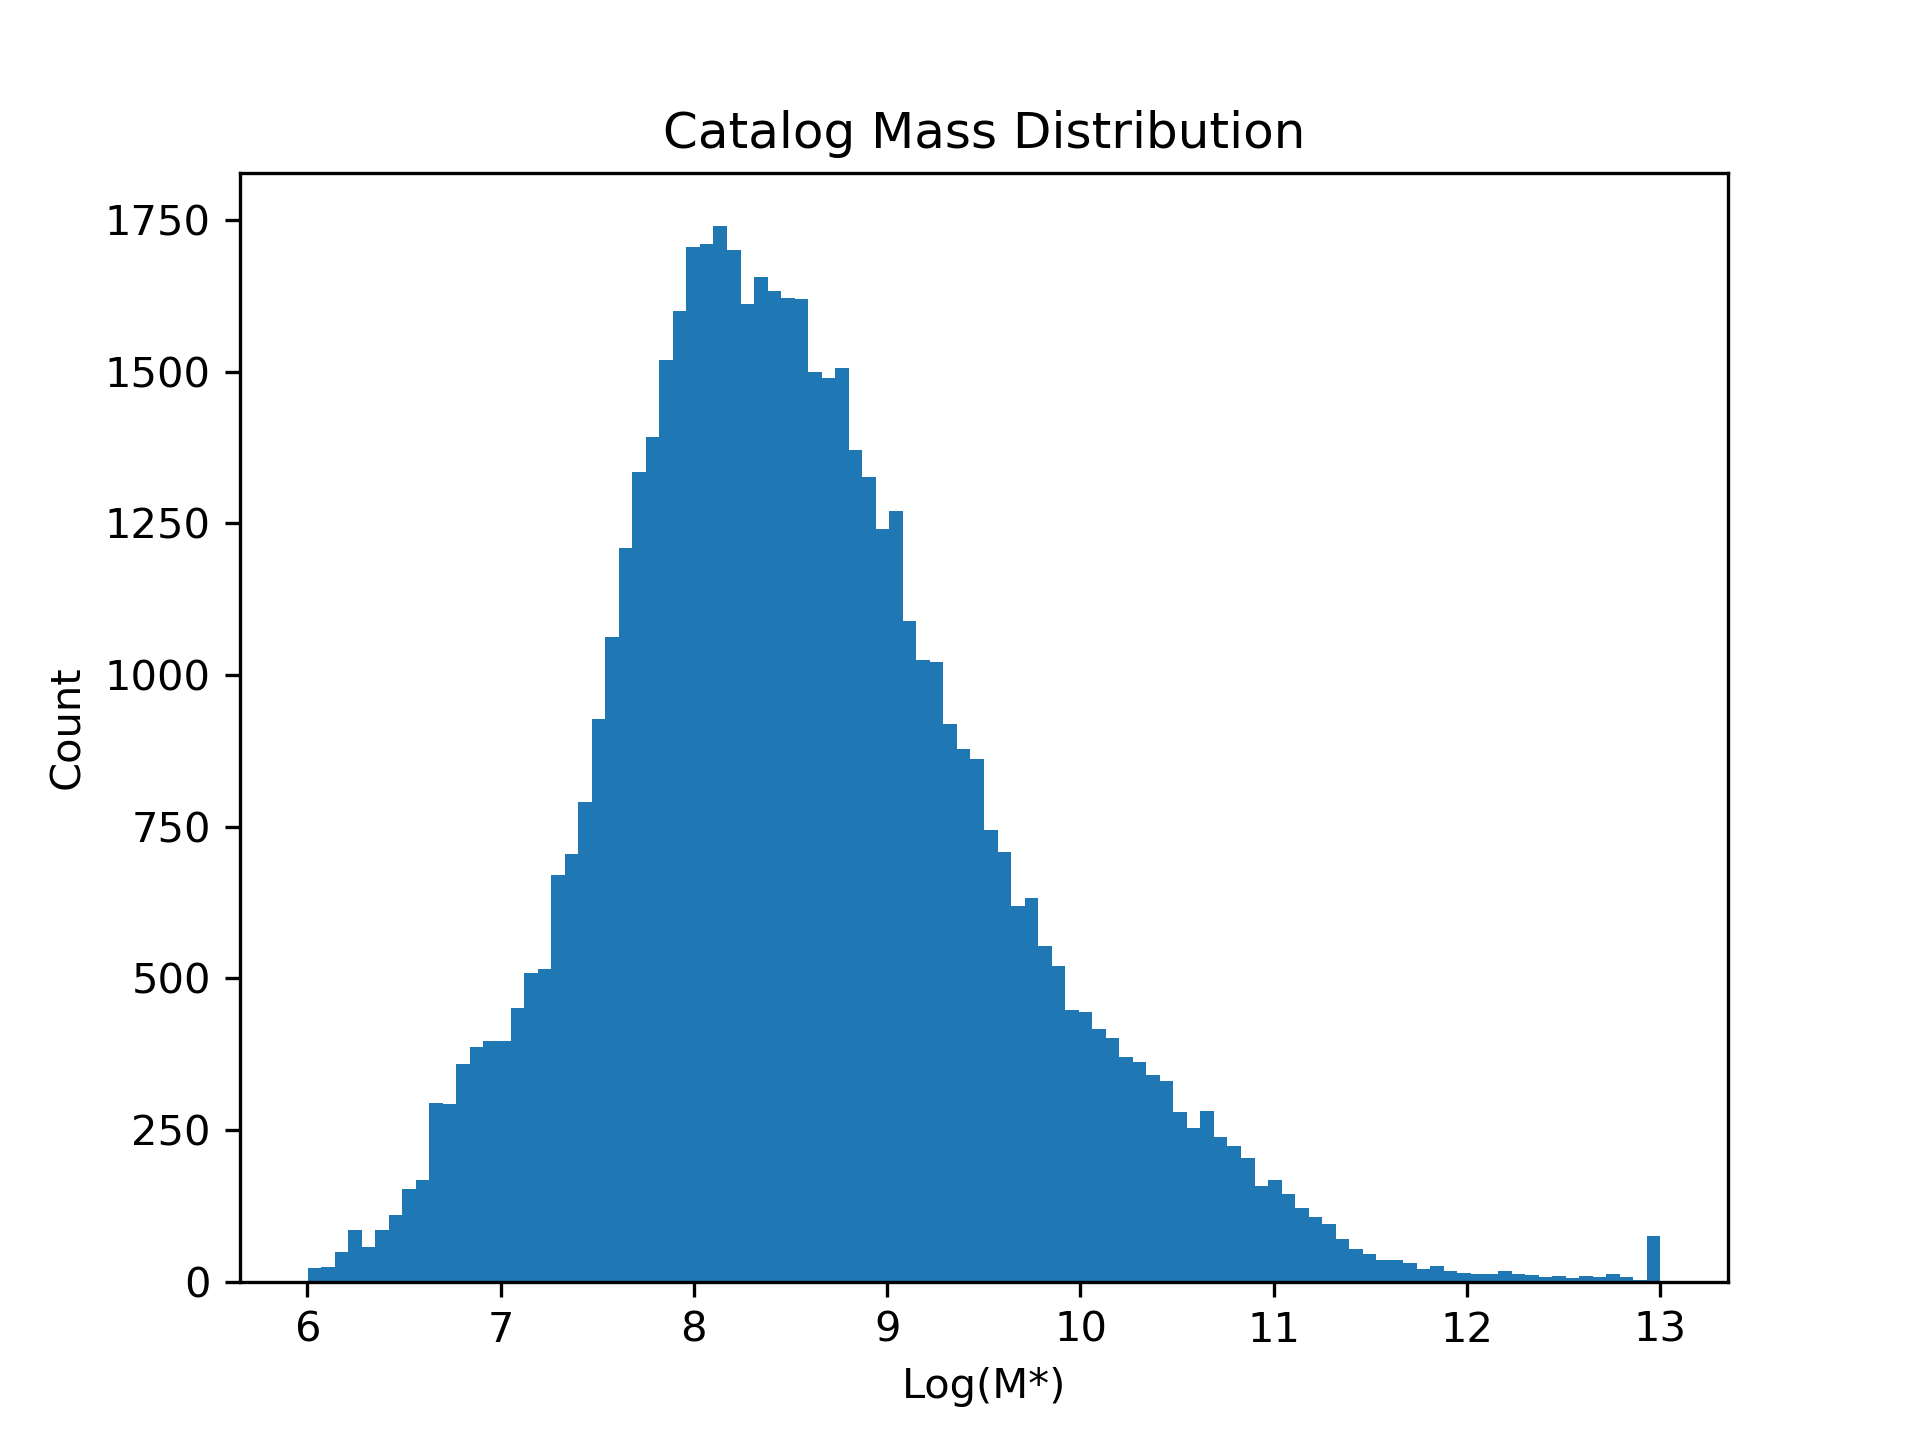
\includegraphics[width=87mm]{Survey/MAGPHYS_Mstar.png}
\caption{Distribution of mass for all galaxies in the catalog. These galaxies have undergone the same quality cut as for the star formation rate plot.}
\label{fig:MAGPHYS_Mstar}
\end{figure}

\section{Method}

As an overview, the method for finding lines, computing the fidelity, cross-matching, and determining matches is the same process as used in the other ASPECS surveys \cite{walter2016alma, decarli2019alma, gonzalez2019alma}.

\subsection{Line Search and Fidelity}

To find possible CO emitters, a search for CO lines was done with the FindClump algorithm first described in \cite{walter2016alma}. This code searches along the spectral axis with different kernel widths in order to maximize the sensitivity to signal associated with line candidates of different intrinsic widths. The widths range from 3 spectral channels up to 19 channels, with each channel being 7.813 MHz wide. The data cubes are searched for lines at any spatial position and spectral coordinate, without any prior based on data from other wavelengths. This is done to minimize any bias in the selection. FindClump returns a list of potential line candidates that then have duplicates removed, which is done by grouping line candidates based on their spatial and spectral position in the cube from each group, only storing the candidate with the highest S/N. This results in 11941 candidates at S/N$>$5.0, 1096 at S/N$>$5.5, 78 at S/N$>$6.0, and 6 at S/N$>$6.5. 

To get a sense of how many of these line candidates are false positives, the fidelity of the lines are then computed. To obtain the fidelity, a line search on the negative data cubes is performed. The negative cubes are obtained by multiplying all the values in each data cube by -1, and rerunning the line search. This catalog of negative lines is then used to compute the fidelity. The fidelity of a line at a given S/N is defined as 

$$ fideltiy(S/N) = 1 - \frac{N_{neg}(S/N)}{N_{pos}(S/N)} $$ where $N_{pos}(S/N)$ and $N_{neg}(S/N)$ are the number of positive and negative line candidates detected at that S/N and for a given line width\cite{gonzalez2019alma}.

The fidelity of the different line widths are shown in Fig. \ref{fig:Fid_map}. As can be seen, the fidelity of the lines is generally higher for wider line widths as more independent resolution elements are included \cite{decarli2019alma}. This means that the S/N cut depends on the width of the line. For example, with a line width of 3 channels, a CO line candidate has to have a S/N $>$ 6.28 to be included in the sample, while for a line candidate with a width of 19 channels, the S/N cutoff is $>$ 6.00. For this report, there were 16 lines at a fidelity $>$0.8, 20 at $>$0.7, 35 at $>$ 0.6, 52 at $>$ 0.5, and 69 at $>$ 0.4. The fidelity cut used for the rest of this analysis is set at 0.6, where every given line has a 60\% chance of being a real line, and leaving us with 35 line candidates. %A breakdown of the number of line candidates as a function of the channel width is shown in Table \ref{table:Fid_NumTable}. 

\begin{figure}[!htbp]
\centering 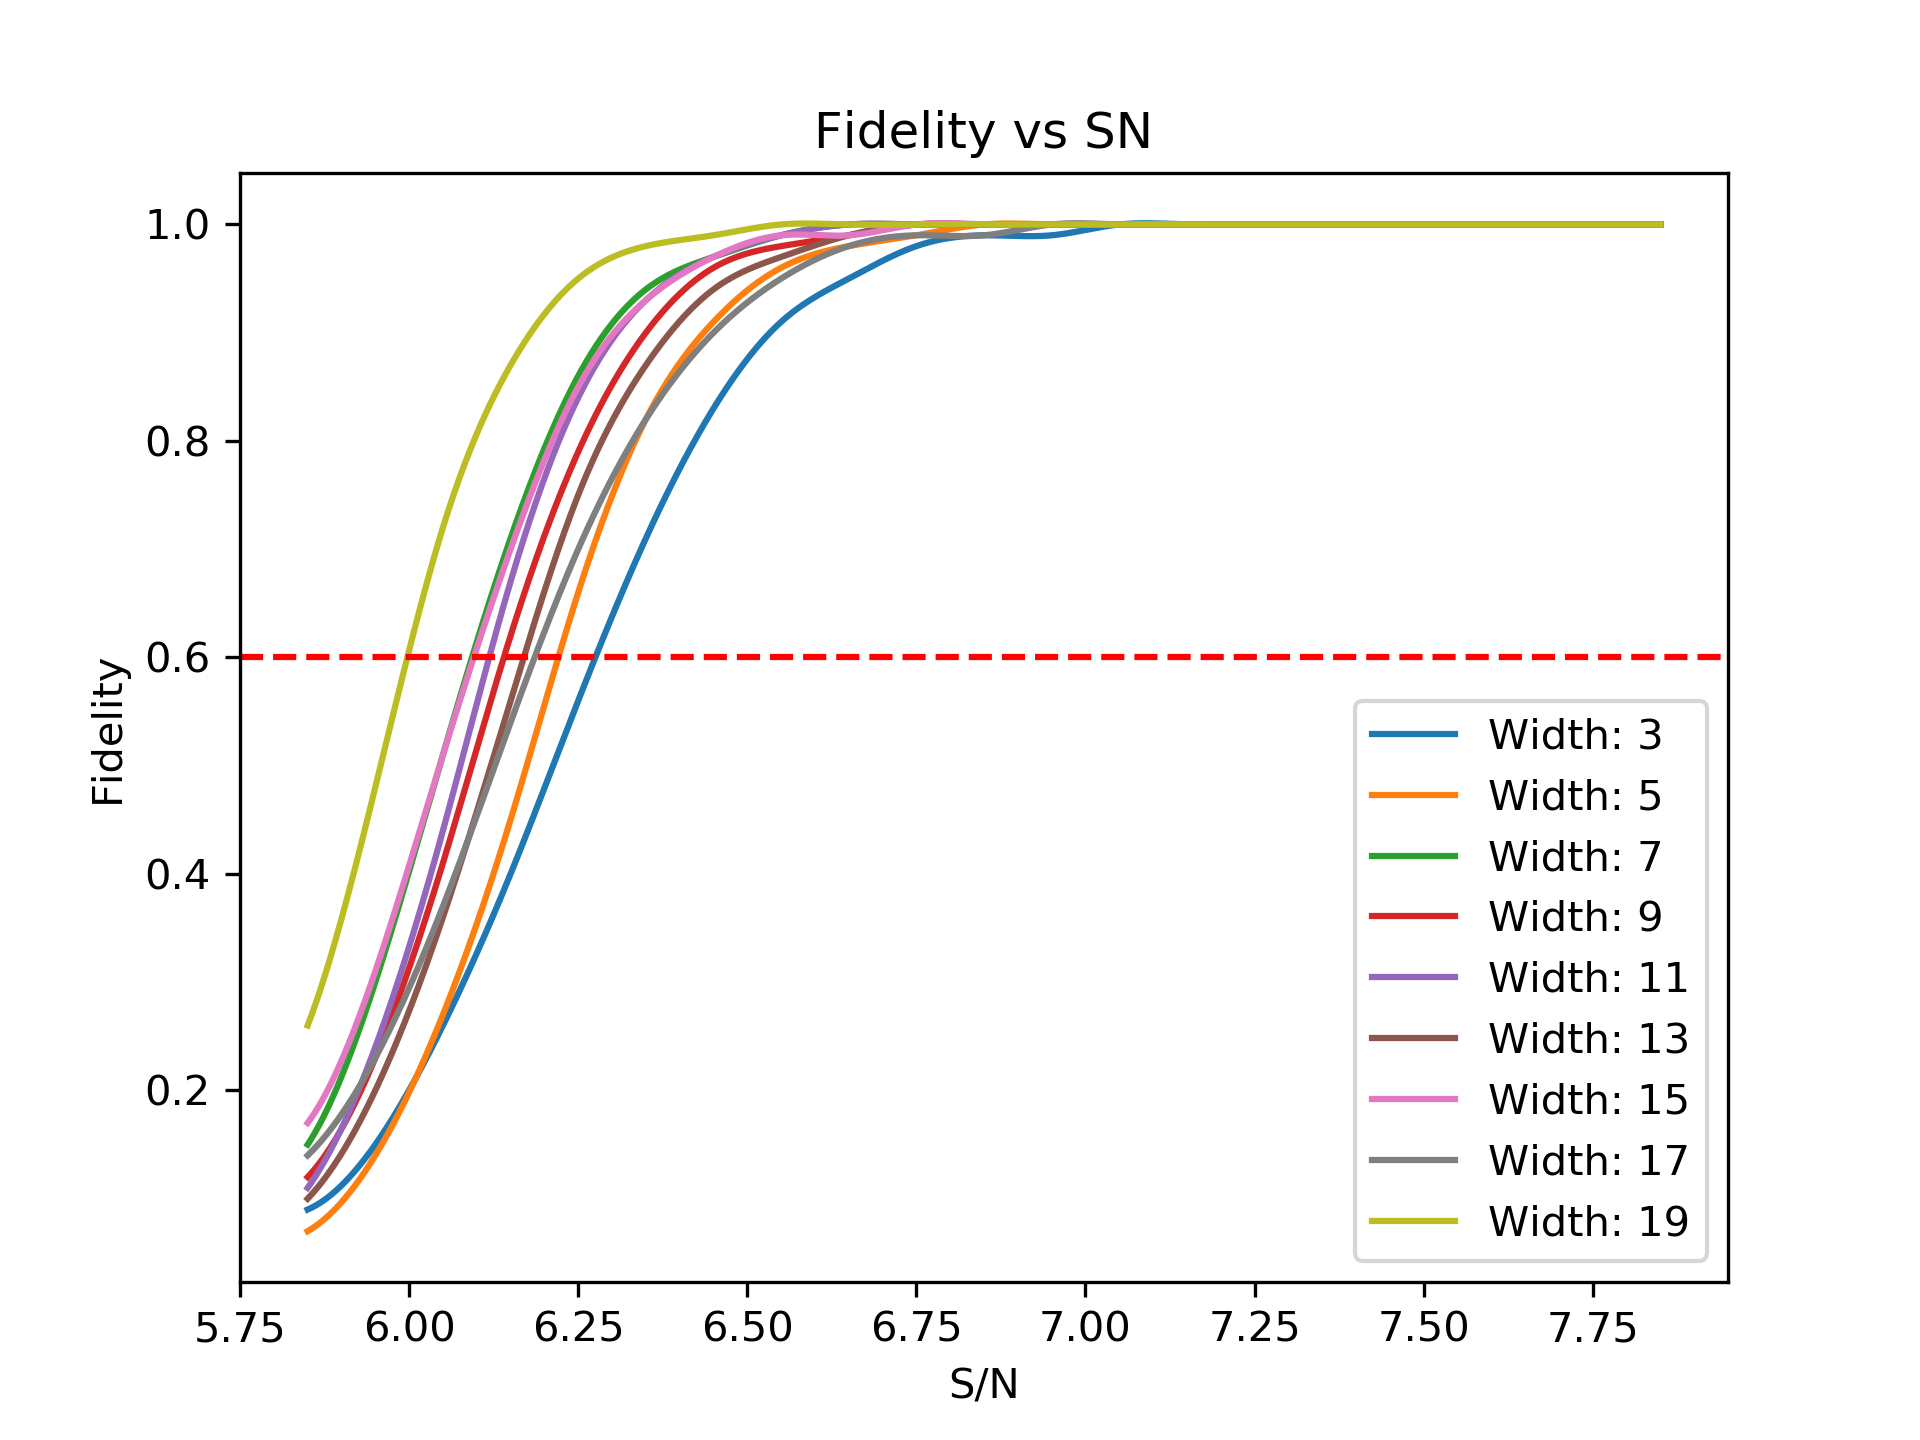
\includegraphics[width=120mm]{Fidelity_map.png}
\caption{Fidelity vs S/N for the different line widths used by FindClump. The red dotted line shows the fidelity = 0.6 cutoff used for the analysis in this report. There are a total of 35 line candidates above that cutoff.}
\label{fig:Fid_map}
\end{figure}

%\begin{table}
%\centering
% its a little confusing how the S/N varies with channel width. May want to explain this in the text. 
%\caption{Number of sources, and S/N cutoffs, per channel width for the adopted fidelity %cut of $>$ 0.6.}\label{table:Fid_NumTable}
%\begin{tabular}{ccc}
%Channels & S/N & N. Sources \\
%\hline
%3 & 6.28 & 3 \\
%5 & 6.22 & 4 \\
%7 & 6.09 & 8 \\
%9 & 6.14 & 2 \\
%11 & 6.12 & 6 \\
%13 & 6.17 & 4 \\
%15 & 6.10 & 3 \\
%17 & 6.19 & 3 \\
%19 & 6.00 & 2 \\
%\end{tabular}
%\end{table}

\subsection{Cross-matching and Redshift Determination}

Once the lines and been found, and the fidelity computed, the next step is to cross-match the CO lines to already known galaxies within the Wide ASPECS footprint. To do this, the spatial location of the line candidates were matched to galaxies that were within one arcsecond of the line candidate's location. Then, assuming that the CO line is from that matched galaxy, the CO transition was calculated. The match was only kept if the offset betwen the CO line's redshift and the galaxy's redshift, $\delta z$, was ($|\delta z| < 0.01$) for galaxies with spectroscopic redshifts, or ($|\delta z| < 0.3$) for ones with photometric redshifts. The differences in $|\delta z|$ thresholds is because spectroscopic redshifts are much more reliable and precise than photometric redshifts. 

If a line matches to more than a single galaxy, then the following steps are performed to differentiate which galaxy the line should be matched to. The first step is to calculate the CO transition for the line assuming the line is matched to each of the galaxies. Once that is determined, the difference in redshift between the CO redshift and the galaxy's redshift is calculated. The matched galaxy that gives the smallest $|\delta z|$, and whose redshift falls within the limits of Wide ASPECS, is then saved as the matched galaxy for that line candidate. 

If there is not a match to a galaxy in the catalog, or if the galaxy's redshift is incompatible with the CO line identification, then the line identification is performed by a bootstrap method, where the probability of a line candidate being one of CO(1-0), CO(2-1), CO(3-2), or CO(4-3) is proportional to the volume of the universe sampled in each of those transitions \cite{walter2016alma, decarli2019alma}.

\section{Results}

The mass versus star formation rate is shown for the general galactic population and the ASPECS sources in Fig. \ref{fig:Cross_match}. For comparison, the Schreiber et al. 2015 \cite{schreiber2015herschel} and Whitaker et al. 2014 \cite{Whitaker_2014} main sequence fits are plotted as well. As can be seen, two of the matched galaxies are above the main sequence and are massive, star-forming galaxies that are the expected type of galaxies for this survey to match to. The other galaxy is much less massive than expected. 

\begin{figure}[!htbp]
% What sample is this? Explain where these 3 matched sources come from when you were talking about 35 above and clarify in the legend that they are all ASPECS matches
\centering 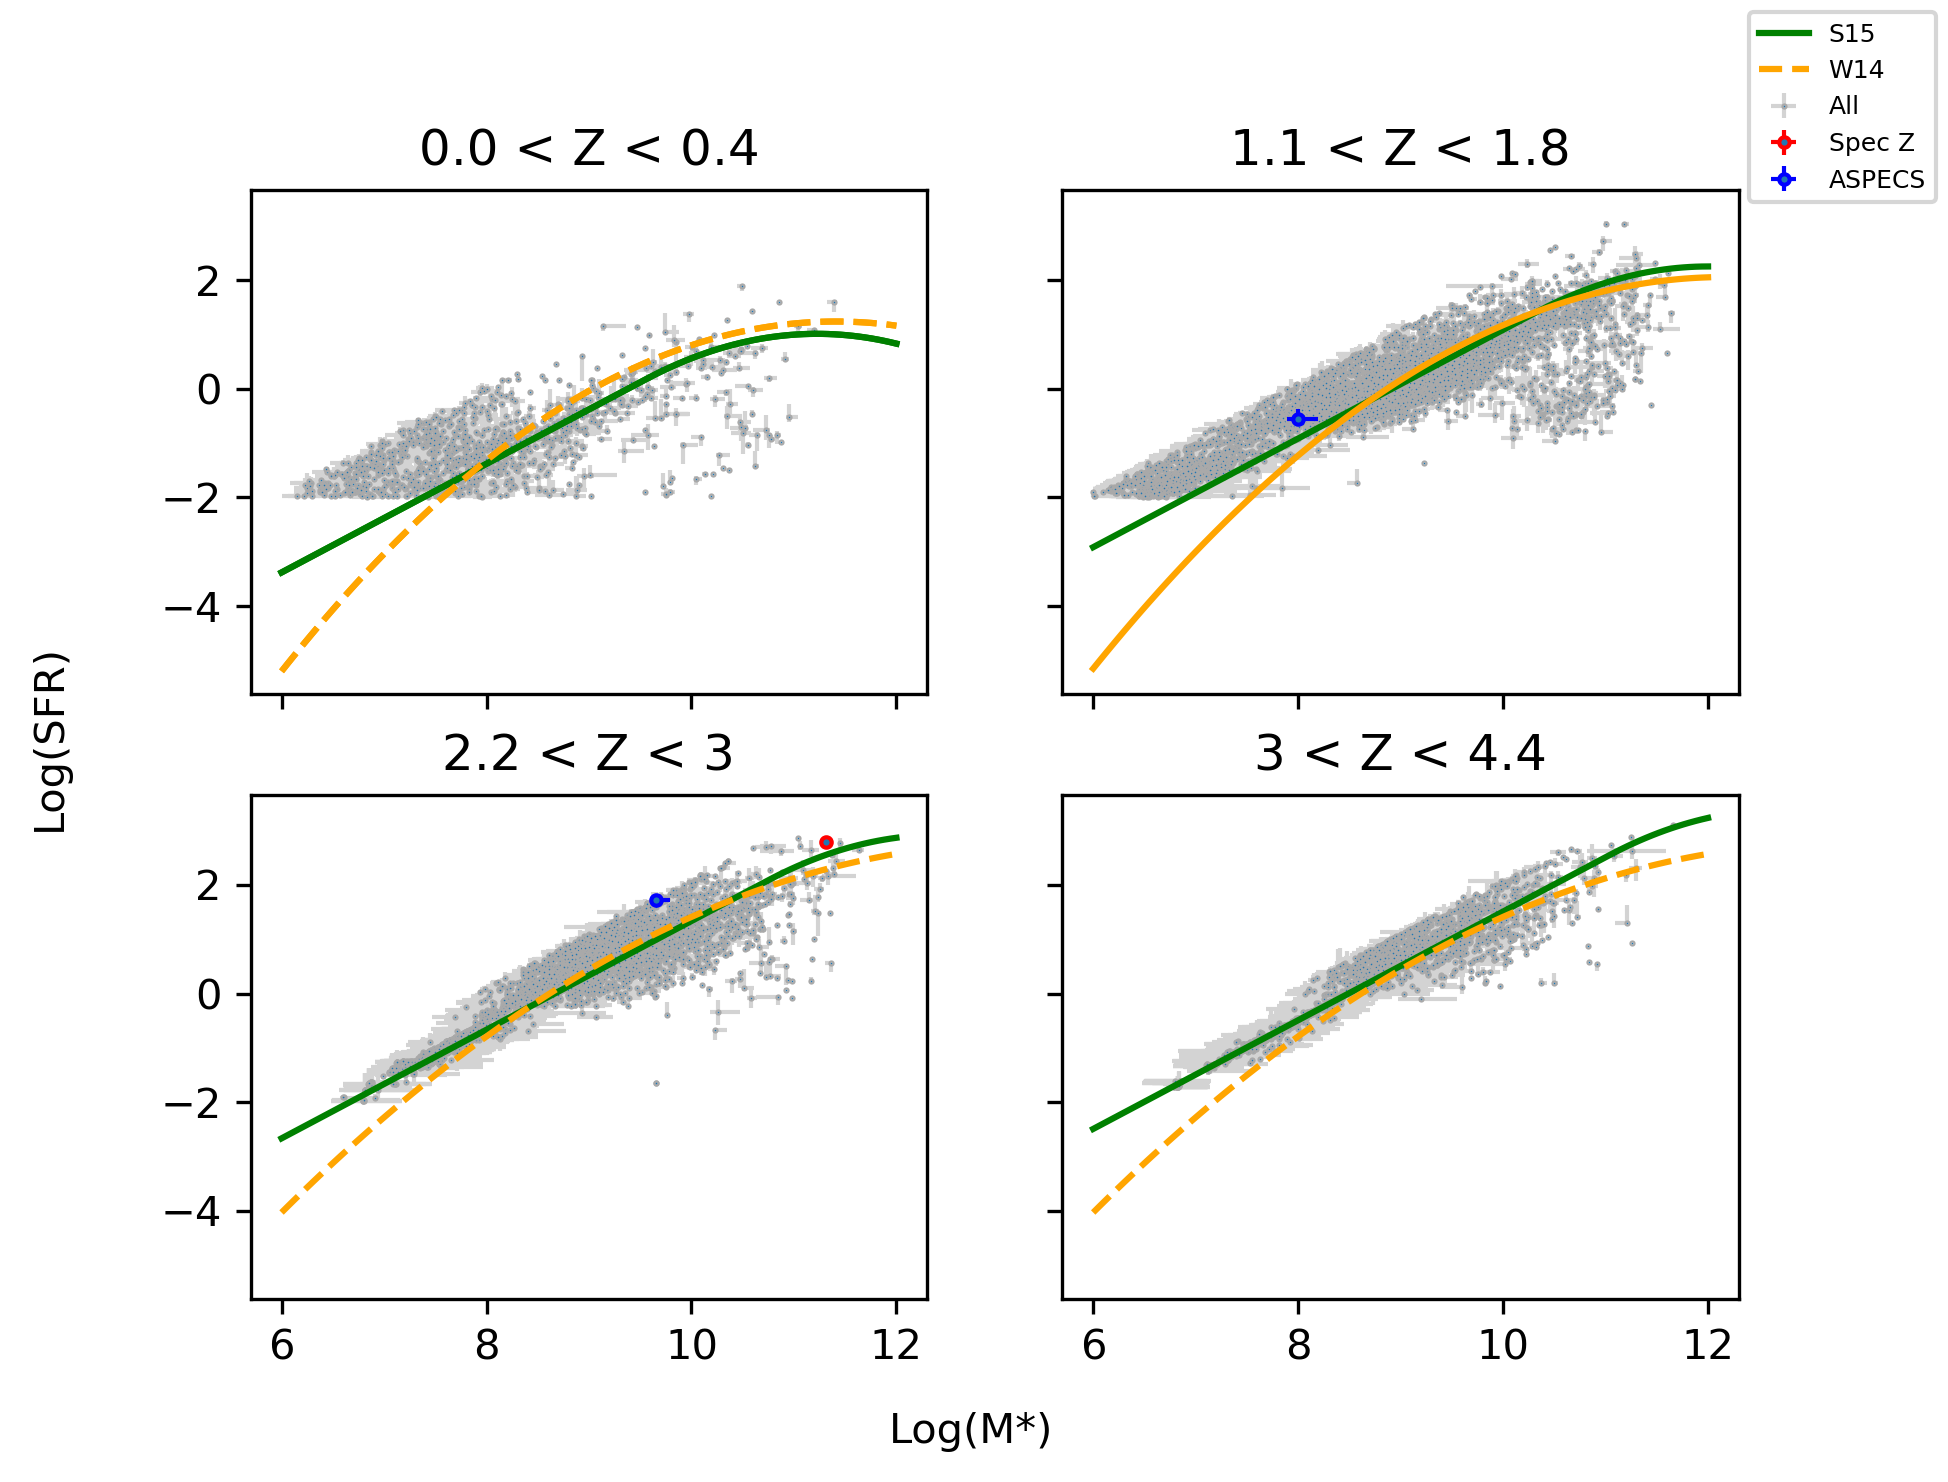
\includegraphics[width=120mm]{Survey/No_Cut_Mstar_vs_SFR_all_closest_sep_1_0_sn_fid_60.png}
\caption{Mass vs Star Formation Rate for galaxies that the fidelity $>$ 0.6 CO line sample matched to. Red points are matched galaxies with spectroscopic redshifts, while blue points are matched galaxies with photometric redshifts. Grey points are all the galaxies in the compiled catalog from \ref{sec:ancillary}. The green lines are the galaxy main sequence fits from \cite{schreiber2015herschel}. The yellow line is from \cite{Whitaker_2014}'s galactic main sequence fit, where the solid line means it is computed within the range mentioned in the paper, while dotted means that the values are extrapolated from the paper to higher, or lower, redshifts. Two of the three matches are on the upper edge of the main sequence, while the third match has a much lower mass and star formation rate than expected for this survey. Error bars are the 16/84th percentile outputs from MAGPHYS.}
\label{fig:Cross_match}
\end{figure}

The final catalog of CO line emitters is shown in Table \ref{table:Catalog}. 3 lines match to galaxies in the catalog. Of those three matches, only ID.1's match has a spectroscopic redshift. The redshift distribution of the whole catalog is shown in Fig. \ref{fig:cat_red}, and some of the physical properties of the three matched lines is shown in Table. \ref{table:matched_gal}. 

\begin{table}[!h]
\centering
% Add table footnotes to explain each column, particularly CO Trans
\caption{The 35 CO line candidates from the fidelity $>$ 0.6 cut.}
\begin{tabular}{ccccccccc}
ID\tablefootnote{Assigned ID for the candidate} & RA\tablefootnote{J2000 system (degrees)} & DEC\tablefootnote{J2000 system (degrees)} & $v_{CO}$\tablefootnote{Observed frequency of the source in GHz.} & CO Tran.\tablefootnote{Estimated CO transition for the line candidate. Goes from $J_{up}$ to $J_{lower}$, e.g. 3-2 is the CO(3-2) transition.} & $z_{CO}$\tablefootnote{Redshift as determined by the CO transition.} & $\delta z$\tablefootnote{Difference in redshift between the CO line transition and the galaxy the line is matched to, if there is one.} & S/N\tablefootnote{Signal-to-noise of the CO line.}& Match?\tablefootnote{If there is a match between the CO line and the galaxy catalog.} \\
\hline
ID.1 & 53.14886 & -27.82118 & 96.701 & 3-2 & 2.576 & 0.006 & 7.31 & Y \\
ID.2 & 53.19145 & -27.76985 & 91.657 & 2-1 & 1.515 & -- & 6.82 & N \\
ID.3 & 53.14138 & -27.84409 & 96.834 & 4-3 & 3.761 & -- & 6.72 & N \\
ID.4 & 53.19242 & -27.78342 & 106.72 & 3-2 & 2.24 & -- & 6.63 & N \\
ID.5 & 53.16066 & -27.76629 & 86.677 & 2-1 & 1.66 & -0.237 & 6.6 & Y \\
ID.6 & 53.16003 & -27.76258 & 103.36 & 3-2 & 2.346 & -- & 6.6 & N \\
ID.7 & 53.13447 & -27.74976 & 102.719 & 3-2 & 2.366 & -- & 6.49 & N \\
ID.8 & 53.11066 & -27.82727 & 85.654 & 3-2 & 3.037 & -- & 6.45 & N \\
ID.9 & 53.11881 & -27.78291 & 104.501 & 3-2 & 2.309 & 0.081 & 6.43 & Y \\
ID.10 & 53.13921 & -27.75352 & 86.67 & 3-2 & 2.99 & -- & 6.43 & N \\
ID.11 & 53.07696 & -27.8251 & 90.891 & 2-1 & 1.536 & -- & 6.42 & N \\
ID.12 & 53.12766 & -27.76666 & 99.553 & 4-3 & 3.631 & -- & 6.42 & N \\
ID.13 & 53.07796 & -27.80182 & 98.725 & 4-3 & 3.67 & -- & 6.36 & N \\
ID.14 & 53.13923 & -27.78228 & 94.407 & 2-1 & 1.442 & -- & 6.35 & N \\
ID.15 & 53.04266 & -27.79322 & 103.173 & 3-2 & 2.352 & -- & 6.3 & N \\
ID.16 & 53.116 & -27.84624 & 97.569 & 4-3 & 3.725 & -- & 6.29 & N \\
ID.17 & 53.09146 & -27.8497 & 106.235 & 3-2 & 2.255 & -- & 6.27 & N \\
ID.18 & 53.18748 & -27.81369 & 89.704 & 1-0 & 0.285 & -- & 6.27 & N \\
ID.19 & 53.11238 & -27.75628 & 88.735 & 3-2 & 2.897 & -- & 6.26 & N \\
ID.20 & 53.12915 & -27.79241 & 91.54 & 2-1 & 1.518 & -- & 6.22 & N \\
ID.21 & 53.1179 & -27.8184 & 92.876 & 2-1 & 1.482 & -- & 6.21 & N \\
ID.22 & 53.06549 & -27.84266 & 104.094 & 3-2 & 2.322 & -- & 6.21 & N \\
ID.23 & 53.1612 & -27.76049 & 94.618 & 2-1 & 1.437 & -- & 6.19 & N \\
ID.24 & 53.11182 & -27.82032 & 99.522 & 4-3 & 3.633 & -- & 6.19 & N \\
ID.25 & 53.07121 & -27.82724 & 88.954 & 3-2 & 2.887 & -- & 6.17 & N \\
ID.26 & 53.19977 & -27.8282 & 100.055 & 3-2 & 2.456 & -- & 6.16 & N \\
ID.27 & 53.06316 & -27.82356 & 84.623 & 3-2 & 3.086 & -- & 6.15 & N \\
ID.28 & 53.09788 & -27.76003 & 90.618 & 3-2 & 2.816 & -- & 6.13 & N \\
ID.29 & 53.16282 & -27.84445 & 90.571 & 3-2 & 2.818 & -- & 6.12 & N \\
ID.30 & 53.09665 & -27.81229 & 95.259 & 2-1 & 1.42 & -- & 6.12 & N \\
ID.31 & 53.13844 & -27.80491 & 102.376 & 3-2 & 2.378 & -- & 6.12 & N \\
ID.32 & 53.16516 & -27.82257 & 104.931 & 3-2 & 2.295 & -- & 6.11 & N \\
ID.33 & 53.19483 & -27.81481 & 98.873 & 4-3 & 3.663 & -- & 6.1 & N \\
ID.34 & 53.08948 & -27.78102 & 86.068 & 3-2 & 3.018 & -- & 6.1 & N \\
ID.35 & 53.14828 & -27.84444 & 87.302 & 3-2 & 2.961 & -- & 6.1 & N \\
\end{tabular}
\end{table}\label{table:Catalog}

\begin{figure}[tbp]
% Need more details. What defines the sample of galaxies shown here? Those above S/N>XX with counterpart matches? Are they photoz/specz?
% Need to add the photo and spec z ones as their own thing
\centering 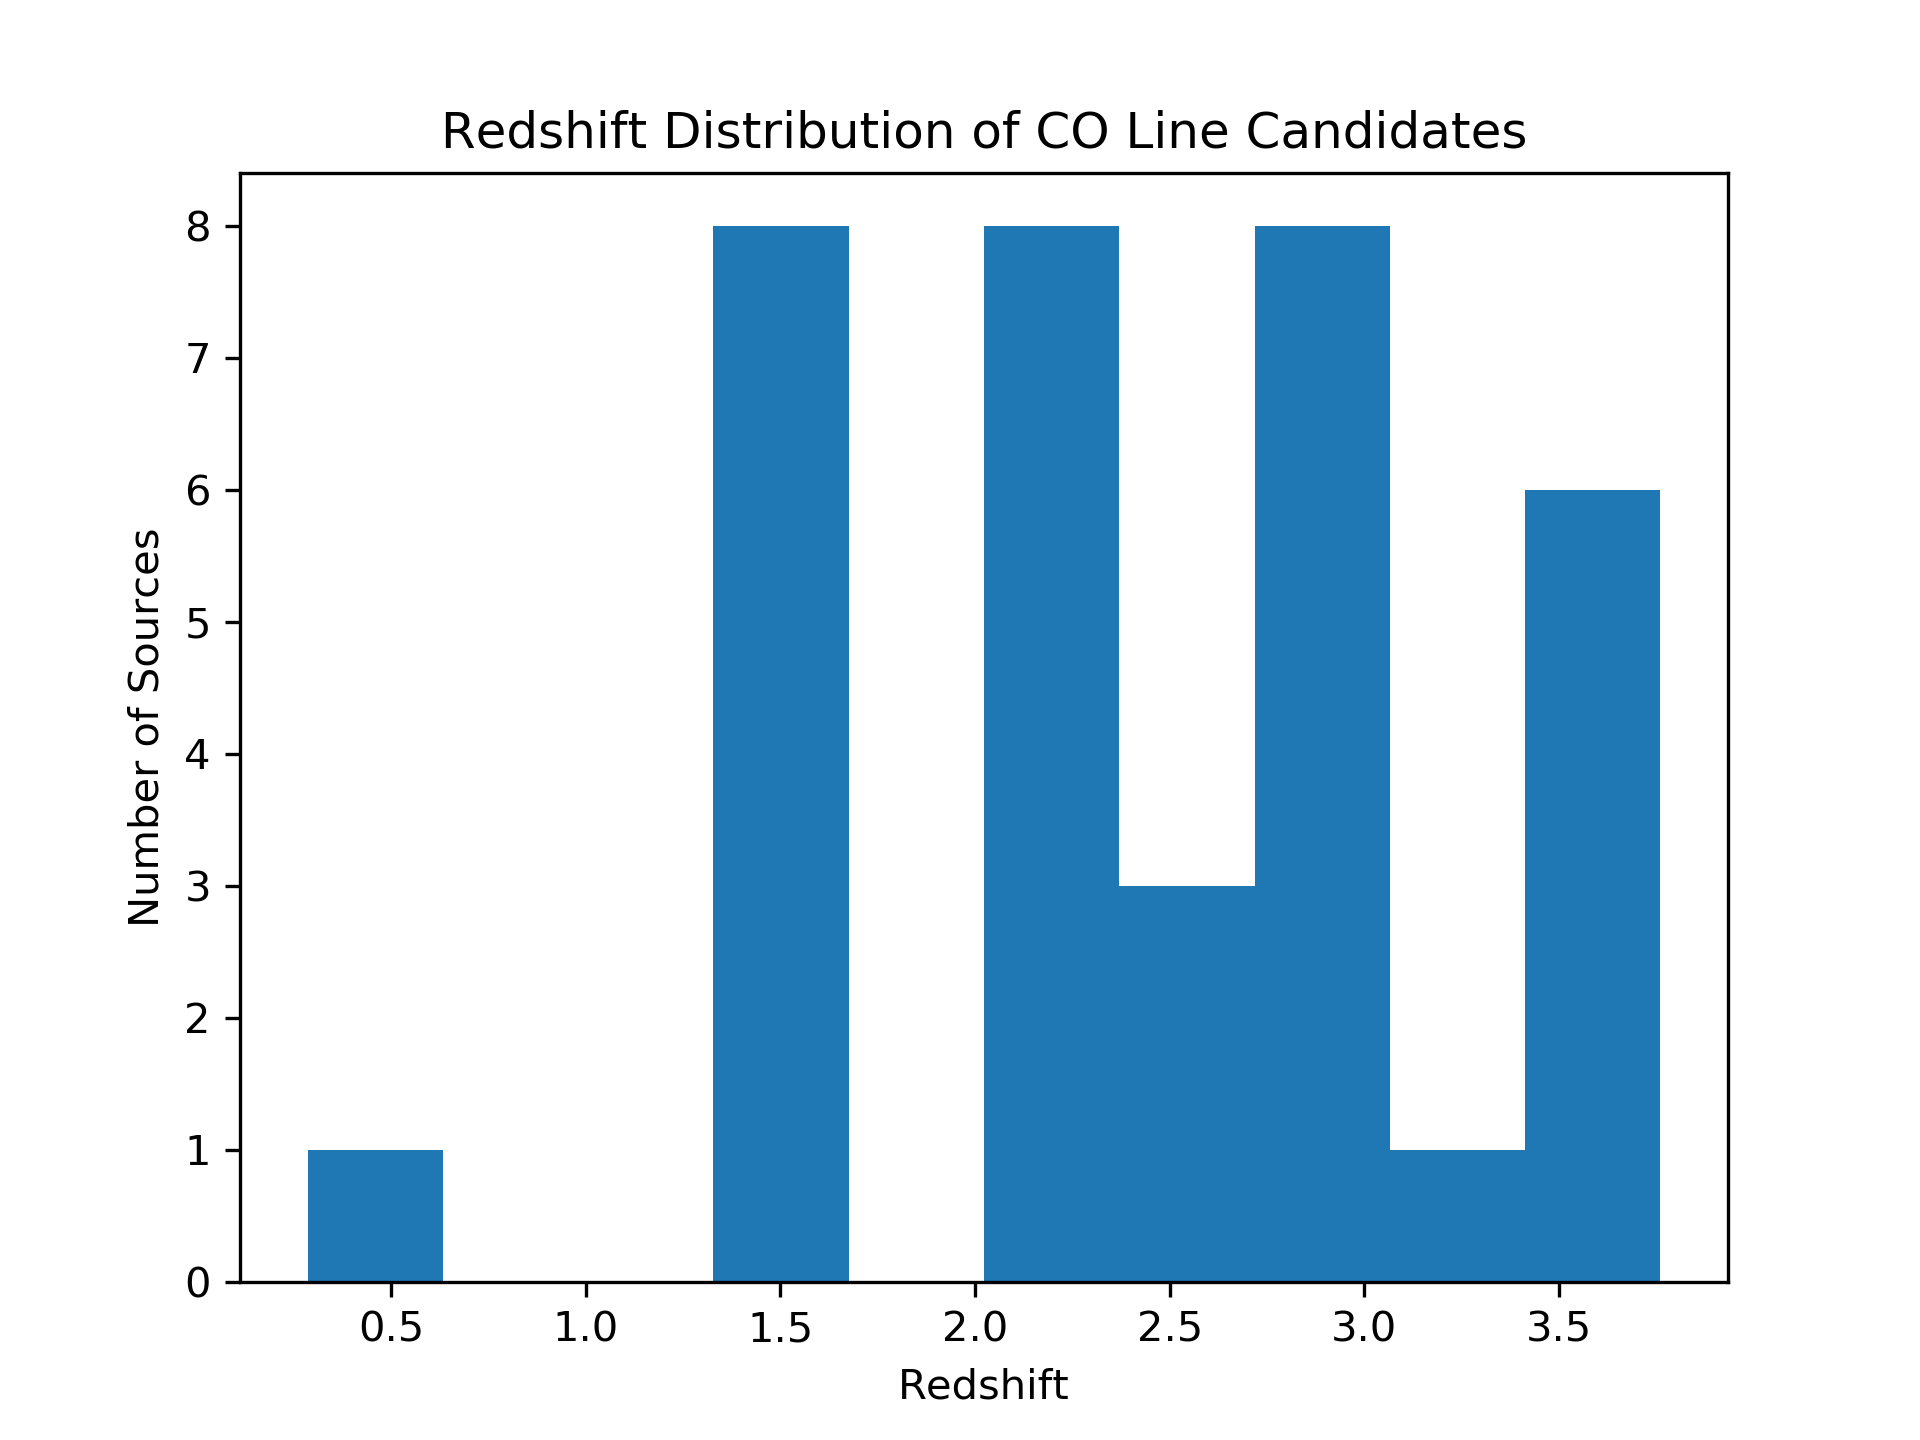
\includegraphics[width=120mm]{Survey/redshift_catalog.png}
\caption{Redshift distribution for all CO line candidate redshifts with a fidelity above 0.6, shown in Table \ref{table:Catalog}. These are the redshifts of the CO lines as determined by matching them to a CO transition, not including the redshifts of the 3 matched galaxies.}
\label{fig:cat_red}
\end{figure}

\begin{table}
% Do these really have 0.0 error on SFR and Mstar?
% TODO: Update the lower limit from MAGPHYS for these.
\caption{This shows some of the physical parameters for the 3 matched line candidates. Sep is the separation in arcseconds between the CO line and the galaxy. $z_{catalog}$ is the master catalog's redshift for the galaxy.}
\begin{tabular}{ccccccccccccccc}
ID & Trans. & $z_{CO}$ & $z_{catalog}$ & $\delta z$ & Spec & S/N & Sep & Log(SFR) & Log(M*) \\
\hline
ID.1 & 3-2 & 2.576 & 2.582 & 0.006 & Y & 7.31 & 0.2824 & $2.782_{-0.005}^{+0.005}$ & $11.31_{-0.0}^{+0.0}$  \\
ID.5 & 2-1 & 1.66 & 1.423 & -0.237 & N & 6.6 & 0.9723 & $-0.453_{-0.115}^{+0.255}$ & $8.017_{-0.105}^{+0.175}$ \\
ID.9 & 3-2 & 2.309 & 2.39 & 0.081 & N & 6.43 & 0.4861 & $1.307_{-0.0}^{+0.0}$ & $9.757_{-0.0}^{+0.0}$ \\
\end{tabular}\label{table:matched_gal}
\end{table}

% Make these in less wavelengths -> smaller too so it fits -> Detail them more here
% In addition, the line candidates are shown overlaid over other wavelengths in the Appendix \ref{sec:A1}.

\section{Discussion}

Of the 35 line candidates chosen for the final catalog, only $~$9\% percent of the lines match to galaxies. Of those that do, only two matched to the most massive, most star forming galaxies in the field.

% Software based explanations

Possible explanations include issues with MAGPHYS' fitting of the galaxies in the catalog, as many of the galaxies seem poorly constrained.

% Physics based explanations

Other possible explanations include the galaxies are very dusty and optically dark, and so have not shown up in shorter wavelengths. Previous ASPECS surveys have found CO candidates without any obvious match to a previously known galaxy, same with the PdBI survey and COLDz. This potentially means that these CO lines without matches are too obscured in other wavelengths to have been detected before. 
% This is just one explanation. What if the galaxies are really dusty and so they just don't show up at shorter wavelengths?